\chapter{Linear Programming and the Simplex Method}\label{app:lp}

Linear programming is a sophisticated technique to explore large, constrained
option spaces to find optimal solutions to systems of equations given some
objective. The seminal paper on linear programming techniques was provided by
Kantorovich in 1940 \cite{kantorovich_new_1940}; however, this occurred during
World War II, and was thus kept secret. An efficient solution technique (called
the Simplex Method was provided by Dantzig in 1947 and published in 1951
\cite{dantzig_maximization_1951}, effectively opening the field. The realm of
linear programming is well studied in the field of optimization
sciences. 

\section{Linear Programming}

Linear programs (LPs) have a relatively simple general construction. There are a
set of $n$ decision variables forming a vector, $x$, a cost vector, $c$, a
constraint matrix, $A$, associated with $m$ constraints and a right-hand-side
threshold vector, $b$. The standard form for linear programs is as follows.

%%% 
\begin{subequations}\label{eqs:std-form}
  \begin{align}
    %%
    \min_{x} \:\: & 
    z = c^{\top} x
    & \label{eqs:std-form_obj} \\
    %%
    \text{s.t.} \:\: &
    A x \geq b 
    & \label{eqs:std-form_sup} \\
    %%
    &
    x \geq 0
    &\label{eqs:std-form_x}
    %%
  \end{align}
\end{subequations}
%%% 

It is important to note that LPs can be formulated in many ways, e.g. as
minimization problems, with equality constraints, etc. Most texts cover the
standard transformations required to turn a given formulation into the standard
form. In general, any LP can be transformed into the standard form.

The $m \times n$ dimensional constraint matrix defines an $n$-dimensional option
space. Any set of values for the vector of decision variables, $x$, that does
not violate a constraint (including those bounding the variables) is termed
a \textit{feasible solution}. It is not only possible, but likely that a given
problem formation has many feasible solutions, in which case any feasible
solution that optimally satisfies the objective function (i.e., provides a
global minimum in the case of the standard form) is termed an \textit{optimal
solution}. It is also possible, for a given set of constraints, for there to be
no feasible solutions and thus no optimal solution. Such a problem formulation
is termed \textit{infeasible}. More commonly, the set of constraints forms
a \textit{feasible region}. Take for example the following formulation:

%%% 
\begin{subequations}\label{eqs:feas}
  \begin{align}
    %%
    \max \:\: & 
    3 x_1 + 2 x_2
    & \label{eqs:feas_obj} \\
    %%
    \text{s.t.} \:\: &
    -2 x_1 + x_2 \leq 1 \\
    %%
    &
    x_1 + x_2 \leq 5 
    & \label{eqs:feas_sup} \\
    %%
    &
    x_1 \in [0, 4]
    &\label{eqs:feas_x1} \\
    %%
    &
    x_2 \geq 0
    &\label{eqs:feas_x2}
    %%
  \end{align}
\end{subequations}
%%% 

which creates the feasible solution space shown in yellow in
Figure \ref{fig:feasible}.

\begin{figure}[H]
  \begin{center}
    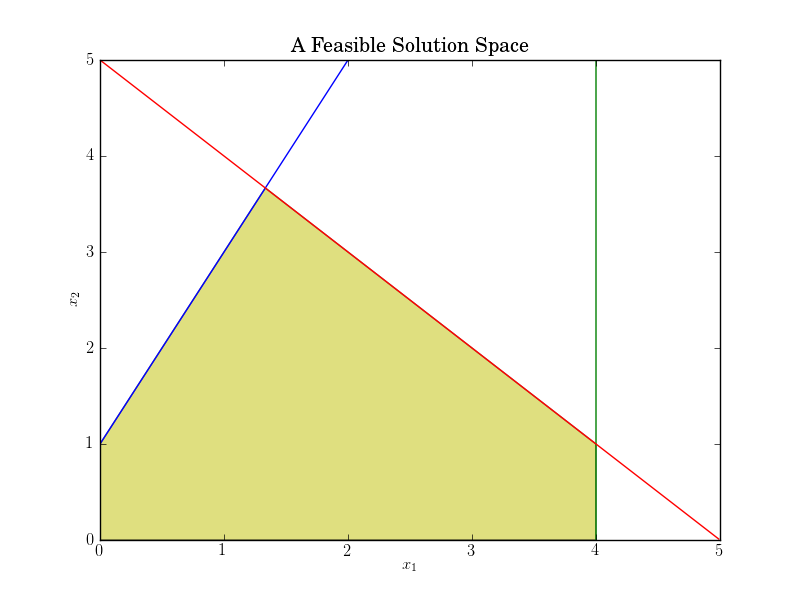
\includegraphics[height=7.5cm]{./backmatter/figs/feasible.png}
  \caption{An example of a feasible solution space.}
  \label{fig:feasible}
  \end{center}
\end{figure}

The program can become infeasible by adjusting a constraint. Take for instance,
an increased boundary constraint for $x_2$.

%%% 
\begin{subequations}\label{eqs:infeas}
  \begin{align}
    %%
    \max \:\: & 
    3 x_1 + 2 x_2
    & \label{eqs:infeas_obj} \\
    %%
    \text{s.t.} \:\: &
    -2 x_1 + x_2 \leq 1 \\
    %%
    &
    x_1 + x_2 \leq 5 
    & \label{eqs:infeas_sup} \\
    %%
    &
    x_1 \in [0, 4]
    &\label{eqs:infeas_x1} \\
    %%
    &
    x_2 \geq 4
    &\label{eqs:infeas_x2}
    %%
  \end{align}
\end{subequations}
%%% 

This arrangement results in the infeasible linear program shown in
Figure \ref{fig:infeasible}, where the updated constraint's effect is shown in
red.

\begin{figure}[H]
  \begin{center}
    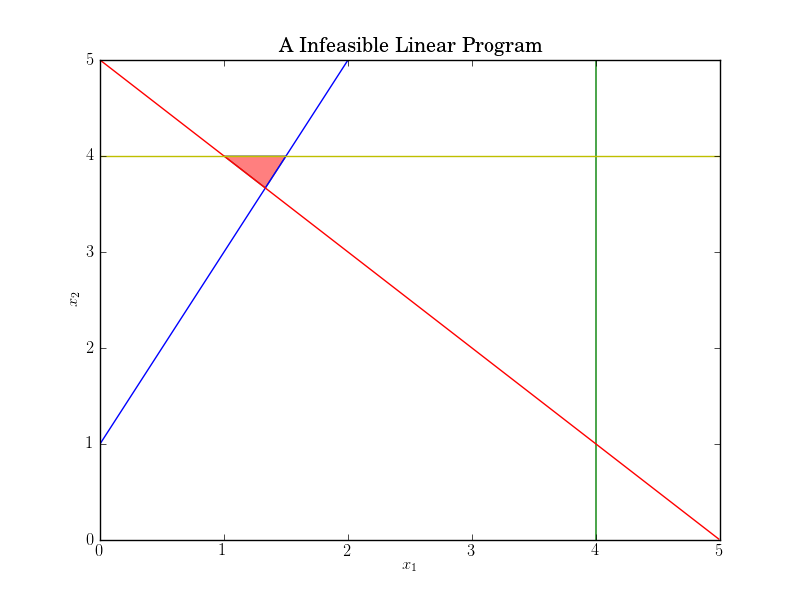
\includegraphics[height=7.5cm]{./backmatter/figs/infeasible.png}
  \caption{An example of a infeasible solution space.}
  \label{fig:infeasible}
  \end{center}
\end{figure}

The standard form of a linear program shown in Equation \ref{eqs:std-form} is an
example of a \textit{primal} linear program. A distinction is made between a
primal linear program and its \textit{dual}. Duality theory is involved and only
treated lightly in this review. The standard form of the dual of Equation
\ref{eqs:std-form} is given in Equation \ref{eqs:dual-form}.

%%% 
\begin{subequations}\label{eqs:dual-form}
  \begin{align}
    %%
    \max_{u} \:\: & 
    w = b^{\top} u
    & \label{eqs:dual-form_obj} \\
    %%
    \text{s.t.} \:\: &
    A^{\top} u \leq c 
    & \label{eqs:dual-form_sup} \\
    %%
    &
    u \geq 0
    &\label{eqs:dual-form_x}
    %%
  \end{align}
\end{subequations}
%%% 

A few critical differences exist. First note that the objective directions are
switched: if a primal form has a minimization objective, its dual has a
maximization objective. The constraint matrix is now $m \times n$-dimensional
(it is in fact the original constraint matrix transposed). There is a new series
of decision variables that form the corresponding solution space, i.e., the
positive vector $u$, as shown in Equation \ref{eqs:dual-form_obj}. These
variables are related to the original right-hand side of the constraint
formulation, the vector $b$. The costs of the original problem, $c$, now form
the right-hand side of the dual's constraint formulation,
Equation \ref{eqs:dual-form_sup}.

The concept of duality is critical in the field of mathematical programming
because it provides well-defined optimality characteristics of a given
program. These are achieved via the \textit{Strong Duality Theorem}
and \textit{Weak Duality Theorem}, shown below as stated
in \cite{ferris_linear_2008}.

\begin{thm}[Weak Duality Theorem]
If $x$ is primal feasible and $u$ is dual feasible, then the dual objective
function evaluated at $u$ is less than or equal to the primal objective function
at $x$.
\end{thm}

The Weak Duality Theorem provides inextricable linkage between a primal feasible
solution and dual feasible solution. If a dual feasible solution is found, it
provides a lower bound on the optimal solution. If a primal feasible solution is
found, it provides an upper bound on the optimal solution. Both of these
criteria, in tandem, help to greatly reduce the required search space during
optimization sweeps.

\begin{thm}[Strong Duality Theorem]
Exactly one of the following three alternatives hold:
\begin{enumerate}

  \item Both primal and dual problems are feasible and consequently both have
  optimal solutions with \textit{equal} extrema

  \item \textit{Exactly one} of the problems is infeasible and consequently the
  other problem has and unbounded objective function in the direction of
  optimization on its feasible region

  \item \textit{Both} primal and dual problems are infeasible

\end{enumerate}
\end{thm}

The Strong Duality Theorem provides the backbone for much of linear programming
theory and application. It states that not only do feasible solutions to the
primal and dual programs provide upper and lower bounds on optimal values, but
that, in fact, the optimal values are \textit{equal}. This provides a criterion
to \textit{know} when an optimal value is reached.

With this slight overview of the realm of linear programming, one can move on to
solution techniques for problems that can be represented as linear programs.

\section{The Simplex Method}

The Simplex Method is a popular algorithm to solve linear programs first
published by Dantzig \cite{dantzig_maximization_1951}. Conceptually, it is quite
intuitive, especially from a geometrical point of view. Before continuing in
more detail, an overview of the method is provided via the example from the
previous section. 

Note that there are five vertices of the polygon (i.e., a polytope more
generally) formed by the full set of constraints:

\begin{enumerate}
  \item $(0, 0)$
  \item $(0, 1)$
  \item $(\frac{4}{3}, \frac{11}{3})$
  \item $(4, 1)$
  \item $(4, 0)$
\end{enumerate}

The Simplex Method begins at a vertex, for example $(0, 0)$, and evaluates the
objective function.

\begin{equation}
    f(0, 0) = 3 * 0 + 2 * 0 = 0 
\end{equation}

Neighbor vertices are then evaluated, in order to determine which provides the
larger value (in the case of maximizing objectives).

\begin{equation}
    f(0, 1) = 3 * 0 + 2 * 1 = 2 
\end{equation}

\begin{equation}
    f(4, 0) = 3 * 4 + 2 * 0 = 12 
\end{equation}

The vertex $(4, 0)$ provides a larger objective function value, so the algorithm
moves to this vertex and determines the next largest neighbor. In this simple
example, there is only one choice, and it is trivially larger.

\begin{equation}
    f(4, 1) = 3 * 4 + 2 * 1 = 14 
\end{equation}

Accordingly the algorithm moves a second time, analyzing the neighboring
vertices again.

\begin{equation}
    f(\frac{4}{3}, \frac{11}{3}) = 3 * \frac{4}{3} + 2 * \frac{11}{3} = \frac{34}{3} 
\end{equation}

At this last move, a terminating condition has been achieved: a vertex has been
found for which all of its neighbors provide a lower value for the objective
function, i.e.,

\begin{equation}
    14 \geq 12 \:\:\: \text{and} \:\:\: 14 \geq \frac{34}{3}.
\end{equation}

Thus, the optimal value for $(x_1, x_2)$ has been determined to be $(4, 1)$. It
is immediately obvious that the simplex algorithm in this state is a hill
climbing (or hill descending) algorithm. The chief reason why this is possible
(i.e., why one is guaranteed to find a globally optimum solution) is that the
objective function and constraints are \textit{convex} functions of the decision
variables. Convexification is required to find optimum solutions to both linear
and integer programs.

In general, the Simplex Method is efficient, i.e., for most cases solutions are
found in less than exponential time in the number of variables. There are
certain program structures for which solution times are exponential, however,
and it in such cases, more advanced \textit{Interior Point} techniques are
required. In general, Interior Point algorithms are often much faster than
Simplex Algorithms \cite{ferris_linear_2008}, but are beyond the scope of this
review.

\subsection{In-Depth Discussion}
To begin a more robust discussion of the Simplex Method, one must introduce the
notion of \textit{slack variables}. Slack variables are used to transform
inequality constraints into equality constraints, effectively taking the
``slack'' out of the system. Slack variables are always positive, thus one could
use a slack variable, $s$, to convert

\begin{equation}
  \sum_{i} a_i x_i \leq b
\end{equation}

to 

\begin{equation}
  \sum_{i} a_i x_i + s = b
\end{equation}

and

\begin{equation}
  \sum_{i} a_i x_i \geq b
\end{equation}

to 

\begin{equation}
  \sum_{i} a_i x_i - s = b.
\end{equation}

The addition of slack variables allows one to rewrite an LP given in the
standard form of Equation \ref{eqs:std-form} as the \textit{canonical form}.

%%% 
\begin{subequations}\label{eqs:can-form}
  \begin{align}
    %%
    \min_{x, s} \:\: & 
    z =  c^{\top} x + 0^{\top} s
    & \label{eqs:can-form_obj} \\
    %%
    \text{s.t.} \:\: &
    A x - b = s
    & \label{eqs:can-form_sup} \\
    %%
    &
    x, s \geq 0
    &\label{eqs:can-form_x}
    %%
  \end{align}
\end{subequations}
%%% 

Given that there are $N$ decision variables and $M$ constraints, the cardinality
of $x$ is $N$ and the cardinality of $s$ is $M$. Furthermore, in the literature,
the $x_i$ variables are termed \textit{nonbasic} variables whereas the $s_i$
variables are termed \textit{basic} variables.

For any LP in the canonical form, the Simplex Algorithm can be applied to it to
determine optimal values for its decision variables, or to determine that it is
unbounded or infeasible. The basic structure of the method is outlined below in
Algorithm \ref{alg:simplex}.

\begin{algorithm}[h!]
 \SetAlgoLined
 \KwData{Decision variables, an objective function, and a set of constraints.}
 \KwResult{Optimal values for the decision variables or a flag denoting 
   infeasibility or unboundedness.}
 Get initial vertex\;
 \If{no vertex is found}{
 feasible solution space is empty\;
 }
 \While{not unbounded and not empty and not done}{ 
    Select column, i, via pricing\;
    \If{no column is found}{
    optimal condition found\;
    done\;
    }
    Select row, j, via the ratio test\;
    \If{no row is found}{
    solution space is unbounded\;
    }
    Perform a Jordan exchange on element (i, j)\;
  }
  \caption{The Simplex Algorithm}\label{alg:simplex}
\end{algorithm}

There are four core operations associated with the Simplex Algorithm:
\begin{enumerate}
  \item finding an initial vertex
  \item column pricing
  \item row selection
  \item exchanging elements
\end{enumerate}

If finding an initial vertex is not trivial (e.g., if the origin is not a
candidate), then the operation to do so requires use of the Simplex Method on a
related LP where the origin is an available candidate. That process will be
described last.

The primary concept required to understand the Simplex Method's operations is
that of the \textit{basis}. The basis begins as the set of decision
variables. The algorithm progresses by moving slack variables into the basis,
and it does so efficiently by analyzing the most ``valuable'' variables to
target (i.e., which current basis variable affects the optimal value the most).

Column pricing and row selection are the operations that select the current
basis and nonbasis variables to target. The Jordan exchange process translates
the formulation into the new basis, exchanging basic and nonbasic
variables. This is perhaps more intuitive from a geometrical point of
view. Consider some starting vertex with many possible sides along which to
move. The process of column pricing and row selection \textit{chooses} the side
along which to move, and the Jordan exchange \textit{reorients} the
problem. Revisiting the example problem, remember the first step. The vertex
$(4, 0)$ was determined to be the best direction in which to move. After a
Jordan exchange, the resulting LP would look like Figure \ref{fig:rotated}.

\begin{figure}[H]
  \begin{center}
    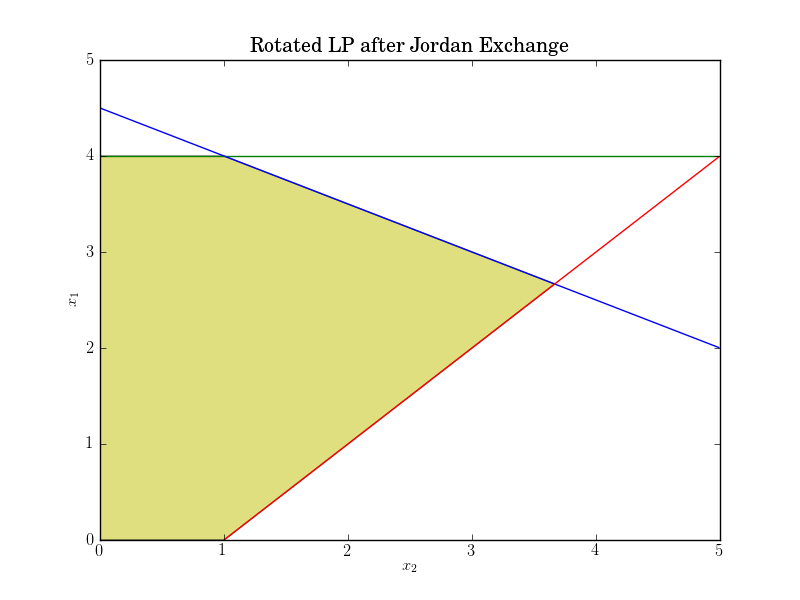
\includegraphics[height=7.5cm]{./backmatter/figs/rotated.png}
  \caption{The Reoriented LP after the first Jordan Exchange.}
  \label{fig:rotated}
  \end{center}
\end{figure}

The column pricing operation selects the slack variable which will enter the
basis. The most naive implementation is to select the variable which will have
the largest effect on the objective function, i.e., which has the largest
magnitude \textit{reduced cost}. For instance, in Equation \ref{eqs:lp_obj},
$x_1$ has a reduced cost of 3, and $x_2$ has a reduced cost of 2 (note that both
costs are in the same positive direction as the objective, i.e.,
maximization). Accordingly, choosing $x_1$ as the nonbasic exchange variable is
a valid option. However, any algorithm may be used to make this selection, as
long as the reduced cost is positive.

Row selection, i.e., selecting the basic variable to enter the basis, is
performed via a ratio test. Given that a column $j$ has been selected, the
corresponding row is selected according to Equation \ref{eqs:ratio-max} in the
case of a maximization objective and Equation \ref{eqs:ratio-min} in the case of
a minimization objective.

\begin{equation}\label{eqs:ratio-max}
  \min \left\{ \frac{-b_i}{A_{i,j}} \:\: | \:\: A_{i,j} > 0 \right\}
\end{equation}

\begin{equation}\label{eqs:ratio-min}
  \min \left\{ \frac{-b_i}{A_{i,j}} \:\: | \:\: A_{i,j} < 0 \right\}
\end{equation}

The Jordan Exchange operation, which transforms a matrix $A \mapsto A'$
given a pivot $(\hat{\imath}, \hat{\jmath})$, is straightforward and is shown in
Equation \ref{eqs:jordan}.

%%% 
\begin{subequations}\label{eqs:jordan}
  \begin{align}
    %%
    a_{\hat{\imath},\hat{\jmath}}' = \frac{1}{a_{\hat{\imath},\hat{\jmath}}}
    &\:\: \text{for} \:
    i = \hat{\imath}, j = \hat{\jmath} \\
    %%
    a_{\hat{\imath},j}' = -\frac{a_{\hat{\imath},j}}{a_{\hat{\imath},\hat{\jmath}}}
    &\:\: \text{for} \:
    i = \hat{\imath}, j \neq \hat{\jmath} \\
    %%
    a_{i,\hat{\jmath}}' = \frac{a_{i,\hat{\jmath}}}{a_{\hat{\imath},\hat{\jmath}}}
    &\:\: \text{for} \:
    i \neq i, j = \hat{\jmath} \\
    %%
    a_{i,j}' = a_{i,j} - a_{i,\hat{\jmath}} a_{\hat{\imath},j}
    &\:\: \text{for} \:
    i \neq \hat{\imath}, j \neq \hat{\jmath}
    %%
  \end{align}
\end{subequations}
%%% 

Finally, one must determine a starting vertex. The original linear program is
modified as shown in \S 3.4 of \cite{ferris_linear_2008}. For each row, $i$, if
$b_i > 0$, then add an additional variable, $x_0$, to the constraint with
coefficient $a_{i,0} = 1$. An initial feasible point is then immediately
available for $x = 0 \:\: \forall \:\: i \neq 0$ and $x_0
= \max(\max(b),0)$. The Simplex Method is then applied, with $x_0$ being the
first variable to leave the basis. When $x_0$ returns to the basis, a suitable
starting vertex results from the removal of $x_0$.
